\documentclass[10pt, t]{beamer}
% \usepackage[UTF8]{ctex}
\usepackage{amsmath}
\usepackage{setspace}
\usepackage{float} 
\usepackage{multido}
\usepackage{multirow}
\usepackage{array}
\usepackage{enumerate}
\usepackage{booktabs}
\usepackage{indentfirst} 
\usepackage[style=mla]{biblatex}
\usepackage{setspace}
\usepackage{subcaption}
\usepackage{hyperref}
\usepackage{textpos}
% \usepackage{fontspec}

% \beamerdefaultoverlayspecification{<+->}
\makeatletter
\let\@@magyar@captionfix\relax
\makeatother

\definecolor{bladerunnerblue}{RGB}{41, 159, 163}
\definecolor{bladerunnerred}{RGB}{194,84,97}
\definecolor{themecolor}{RGB}{25,25,112} 
\definecolor{weak}{RGB}{150,150,150}

\renewcommand{\emph}[1]{{\color{themecolor}\textsl{#1}}}
\newcommand{\alarm}[1]{{\color{bladerunnerred}{#1}}}
\newcommand{\N}{\mathbb{N}}
\newcommand{\R}{\mathbb{R}}
\newcommand{\dom}{\operatorname{dom}}
\newcommand{\myseries}[2]{$#1_1,#1_2,\dots,#1_#2$}
\newcommand{\nullspace}{~\\[15pt]}
\newcommand{\remark}{\textbf{Remark: }}
\newcommand{\question}{\textbf{Question: }}
\newcommand{\scp}[2]{\langle\,#1\,,\,#2\,\rangle} \newcommand{\scpp}{\langle\,\cdot\,,\,\cdot\,\rangle}
\newcommand{\weaken}[1]{{\color{weak}\textit{#1}}}
\newcommand{\underover}[3]{\underset{#2}{\overset{#3}{#1}}}
\renewcommand{\emptyset}{\varnothing}


\usetheme{Madrid}
\setbeamertemplate{navigation symbols}{}

\addtobeamertemplate{frametitle}{}{
\begin{textblock*}{100mm}(0.85\textwidth,-1cm)
\includegraphics[height=1cm]{../../logo.png}
\end{textblock*}}


\usecolortheme[named=themecolor]{structure}

\setbeamertemplate{items}[default]

\hypersetup{
    colorlinks=true,
    linkcolor=themecolor,
    filecolor=themecolor,      
    urlcolor=themecolor,
    citecolor=themecolor,
}

\title{VV186: Honors Mathematics}
\subtitle{Vector Space \& Sequence of Real Functions}
\institute[UM-SJTU JI]{Univerity of Michigan-Shanghai Jiao Tong University Joint Institute}
\author{Xingjian Zhang}

\begin{document}

\begin{frame}
    \titlepage
    \begin{center}
        \includegraphics[height=2cm]{../../logo2.png}
    \end{center}
\end{frame}

\begin{frame}
    \frametitle{Outline}
    \begin{spacing}{1}
        \tableofcontents
    \end{spacing}
\end{frame}

\section{Vector Space}
\begin{frame}[allowframebreaks]
    \frametitle{Vector Space}
    \begin{figure}[H]
        \centering
        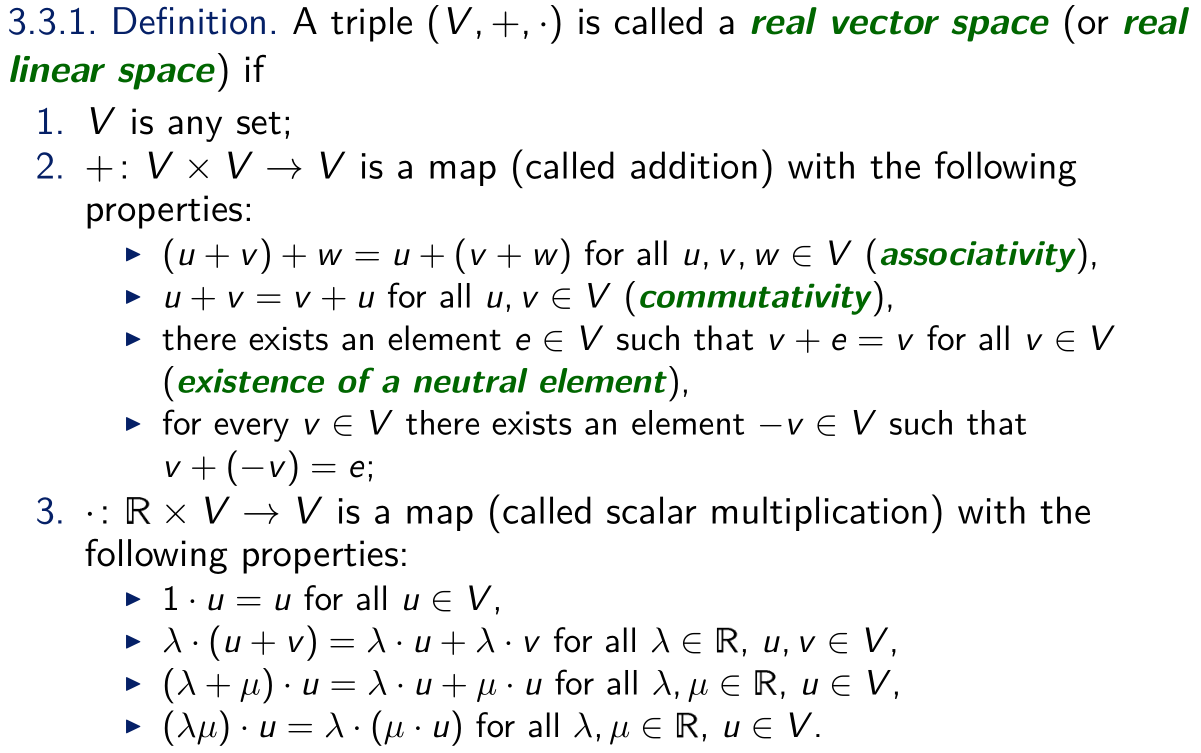
\includegraphics[width=0.9\textwidth]{2020-11-17-19-48-09.png}
    \end{figure}
    \textbf{Remark:}
    \begin{itemize}
        \item 
        Remember all of the 9 properties in the definition.
        \item For both of ``$+$'' and ``$\cdot$'', the \emph{codomain} is $V$. i.e. Both operators should map into original set $V$.
        \item Distinguish clearly a \emph{complex} and a \emph{real} vector space. It is determined by the \emph{domain} of \emph{scalar multiplication}. (Is $\mathbb{C}^n$ a complex or a real vector space?) 
        \item Some common notation:\begin{enumerate}
            \item $\R^n$
            \item $\mathbb{C}^n$
            \item $\mathcal{P}_n$
            \item $C(\Omega , \R)$
            \item $C^k(\Omega , \R)$
            \item $C^\infty(\Omega , \R)$
            \item $\ell^\infty$
            \item $c_0$\footnote[frame]{See Slide p.340 if you forget them.}
        \end{enumerate}
    \end{itemize}
\end{frame}

\begin{frame}
    \frametitle{Subspace}

    We defined the \emph{subspace}:
    \begin{figure}[H]
        \centering
        
\includegraphics[width=0.9\textwidth]{2020-11-17-20-03-23.png}
    \end{figure}

    We have a simple way to verify a candidate $(U,+,\cdot)$ is indeed a subspace of $(V,+,\cdot)$, given that $(V,+,\cdot)$ is a vector space:
    \begin{figure}[H]
        \centering
        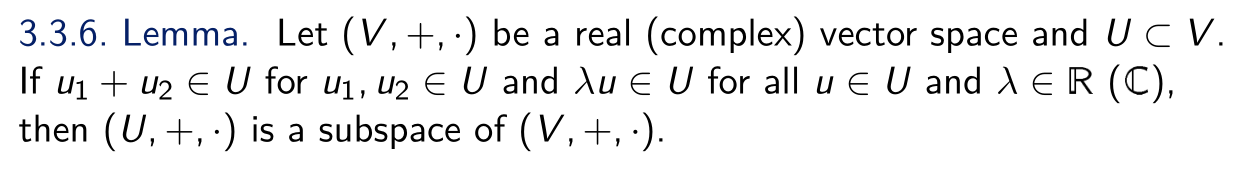
\includegraphics[width=0.9\textwidth]{2020-11-17-20-07-20.png}
    \end{figure}
\end{frame}

\begin{frame}[allowframebreaks]
    \frametitle{Normed Vector Space}

    \emph{Norm} is the ``generalized length function'' in a vector space. We defined it by three properties: 
    \begin{figure}[H]
        \centering
        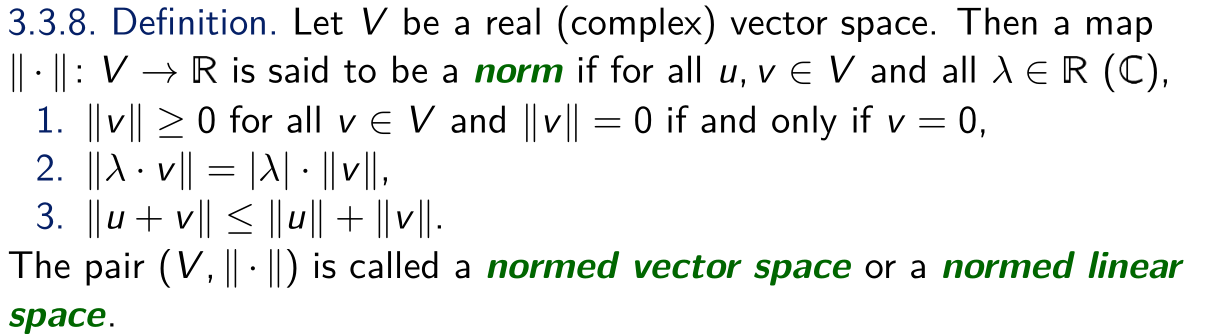
\includegraphics[width=0.9\textwidth]{2020-11-17-20-13-44.png}
    \end{figure}
    \textbf{Remark:}\begin{itemize}
        \item A norm is a (unary) function. So we can naturally investigate into it as considering a function. (e.g. How to prove a norm is continous?)
        \item Any normed vector space can also be considered as a metric space. (How should we define the metric $\rho(x,y)$ according to $\|\cdot\|$?)
        \item Some common notation:\begin{enumerate}
            \item $\|x\|_2$ in $\R^n$ (Euclidean norm)
            \item $\|x\|_p$ in $\R^n$ for $p\in\N^+$
            \item $\|x\|_\infty$ in $\R^n$
            \item $\|(a_n)\|_\infty$ in $\ell^\infty$ or $c_0$
            \item $\|f\|_\infty$ in $C([a,b])$
        \end{enumerate}
    \end{itemize}
\end{frame}

\section{Sequences of Functions}

\begin{frame}
    \frametitle{Pointwise vs. Uniform Convergence}

    \begin{figure}[H]
        \centering
        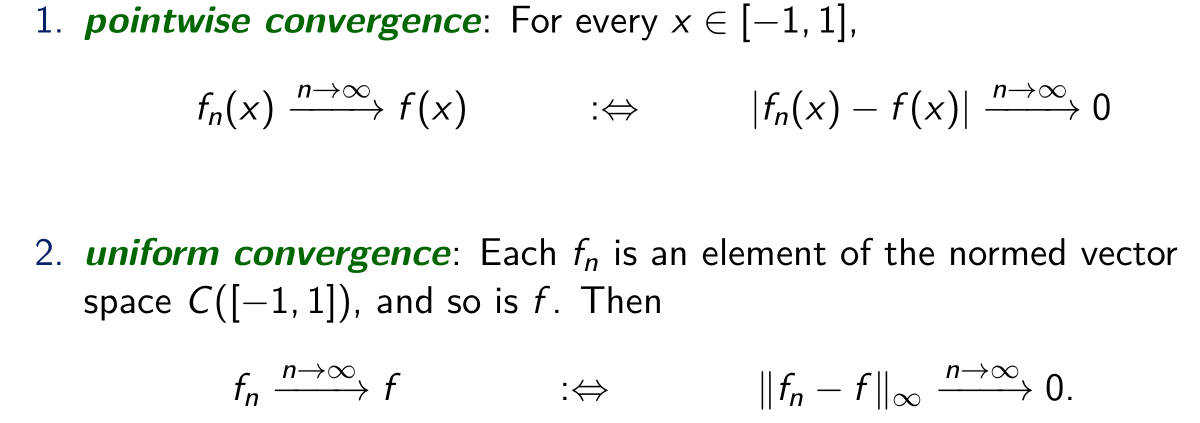
\includegraphics[width=0.9\textwidth]{2020-11-17-20-25-28.png}
    \end{figure}
    \textbf{Remark:}
    \begin{itemize}
        \item What are the differences between two convergence?
        \item What are the relations between two convergence?
        \item Can you come up with some examples to illustrate them?
    \end{itemize}

\end{frame}

\begin{frame}
    \frametitle{End}
    \vspace{2.2cm}
    \begin{center}
        \Large
        Have Fun \\
        And \\
        Learn Well!
    \end{center}
\end{frame}

\end{document}